\chapter{Kodierung}
\section{Notwendigkeit}
\label{sec:notwendigkeit}
Nacheinander gesendete Nibble müssen auf der Leitung voneinander unterscheidbar sein. Um dies zu gewährleisten, wird ein Taktsignal in den Datenstrom kodiert, indem verhindert wird, dass ein gesendetes Nibble gleich seinem Vorgänger ist. Dies verursacht den Sonderfall zweier gleicher aufeinanderfolgender Nibble. Zu dessen Behandlung muss eine Escape-Sequenz definiert werden, welche die gleichen Nibble durchbricht. Durch die Einführung einer solchen Escape-Sequenz wird ihr eigenes Auftreten im Datenstrom jedoch selbst zu einem Sonderfall. Zur Handhabung dieser Sonderfälle und zur Kennzeichnung von Blöcken wird ein Protokoll zwischen Sender und Empfänger vereinbart.

\section{Besondere Sequenzen}
Aus den in Abschnitt \ref{sec:notwendigkeit} dargelegten Gründen werden vordefinierte Sequenzen in den Datenstrom injiziert. Eine solche Sequenz setzt sich aus vier festen (Escape-Sequenz) und vier dynamischen Bits (Handlungsanweisung: "Command") zusammen. Alle verwendeten 4 Bit Sequenzen sind in Tabelle \ref{tab:escape_sequences} gelistet und in ihrer Funktion erläutert.

\begin{figure}[H]
    \centering
    \[
        \underbrace{\text{XXXX}}_\text{\normalsize esc} \ \overbrace{\text{XXXX}}^\text{\normalsize cmd}
    \]
    \caption{Aufbau einer Kodierungssequenz}
\end{figure}

Die \textbf{Escape-Sequenz} trennt kodierende Sequenzen vom restlichen Datenstrom ab. Sie selbst hält keine Information darüber, um welche Kodierung es sich handelt. Aufgrund ihrer Sonderfunktion darf sie nicht regulär im Datenstrom auftreten und muss ggf. selbst escaped werden.

\textbf{Commands} erhalten erst dann ihre Bedeutung, wenn sie unmittelbar nach der Escape-Sequenz stehen. Sie geben Auskunft darüber, um welche Kodierung es sich handelt und implizieren, wie sich ein Dekodierender verhalten muss, um die originalen Daten wieder zu rekonstruieren. Ist das nachfolgende Nibble auf einen Command (im binären) mit diesem identisch, wird anstelle des normalen Commands dessen Fallback-Version genutzt.

\begin{table}[H]
    \center
    \def\arraystretch{1.3}
    \rowcolors{2}{gray!15}{white}
    \begin{tabular}{|c|l|l|}
        \rowcolor{gray!50}
        \hline
        \textbf{Hex} & \textbf{Bezeichnung}          & \textbf{Bedeutung}                 \\
        \hline
        0            & escapeSequence                & Das nächste Nibble ist ein Command \\
        1            & beginDataBlockDefault         & Ein Datenblock beginnt             \\
        2            & beginDataBlockFallback        & Ein Datenblock beginnt             \\
        3            & beginControlBlockDefault      & Ein Kontrollblock beginnt          \\
        4            & beginControlBlockFallback     & Ein Kontrollblock beginnt          \\
        5            & endBlockDefault               & Der aktuelle Block endet           \\
        a            & endBlockFallback              & Der aktuelle Block endet           \\
        6            & insertPrevNibbleAgainDefault  & Ein doppeltes Nibble im Datenstrom \\
        7            & insertPrevNibbleAgainFallback & Ein doppeltes Nibble im Datenstrom \\
        8            & insertEscSeqAsDataDefault     & Die Esc-Seq trat im Datenstrom auf \\
        9            & insertEscSeqAsDataFallback    & Die Esc-Seq trat im Datenstrom auf \\
        \hline
    \end{tabular}
    \caption{Bitsequenzen und ihre Bedeutung}
    \label{tab:escape_sequences}
\end{table}

\section{Datenblöcke}
Datenblöcke dienen zur Übertragung der Rohdaten. Da gemäß Aufgabenstellung bis zu 1GB große Dateien zu senden sind und maximal 64 Byte pro Paket übertragen werden, ist die Paket-ID $\lceil \log_{2}{(1\text{GB} / 64 \text{B})} \rceil = 24$ Bit lang. Der Aufbau eines Datenpakets ist in Abbildung \ref{fig:datapacket} dargestellt. Die Länge des gesamten Paketes ist wegen der Kodierung zur Laufzeit möglicherweise größer, als dort abgebildet.
\vspace{0.5cm}

\begin{figure}[H]
    \centering
    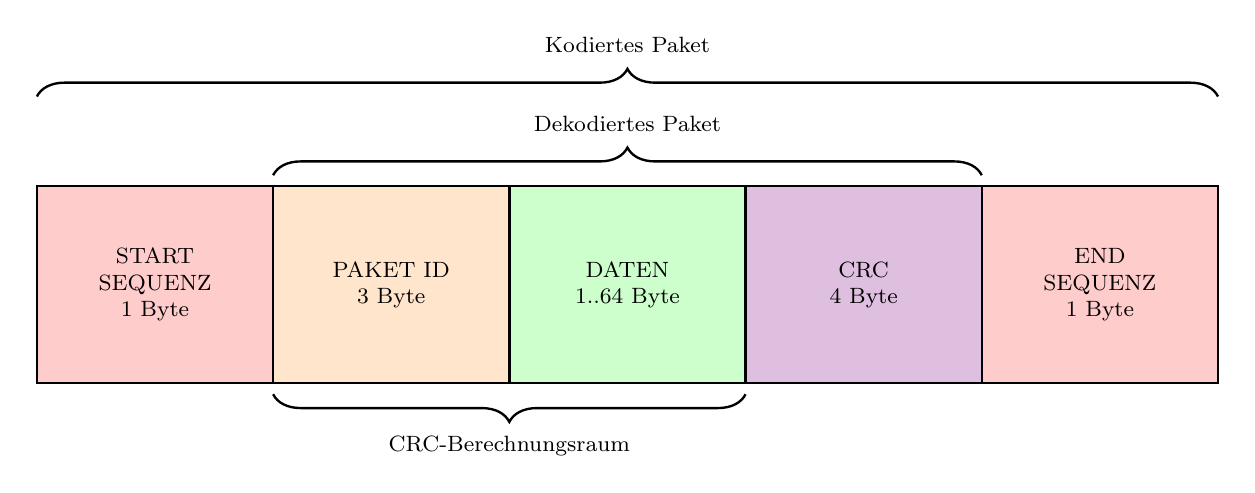
\begin{tikzpicture}[every node/.style={font=\footnotesize},every path/.style={line width=0.3mm}]

        \draw[fill=red!20] (0,0) rectangle (3,2.5) node[midway] {\parbox{3cm}{\centering START\\SEQUENZ\\1 Byte}};
        \draw[fill=orange!20] (3,0) rectangle (6,2.5) node[midway] {\parbox{3cm}{\centering PAKET ID\\3 Byte}};
        \draw[fill=green!20] (6,0) rectangle (9,2.5) node[midway] {\parbox{3cm}{\centering DATEN\\1..64 Byte}};
        \draw[fill=violet!25] (9,0) rectangle (12,2.5) node[midway] {\parbox{3cm}{\centering CRC\\4 Byte}};
        \draw[fill=red!20] (12,0) rectangle (15,2.5) node[midway] {\parbox{3cm}{\centering END\\SEQUENZ\\1 Byte}};

        \draw [decorate,decoration={brace,amplitude=10pt,raise=4pt},yshift=1cm]
        (0,2.5) -- (15,2.5) node [black,midway,yshift=0.8cm] {Kodiertes Paket};
        \draw [decorate,decoration={brace,amplitude=10pt,raise=4pt},yshift=0pt]
        (3,2.5) -- (12,2.5) node [black,midway,yshift=0.8cm] {Dekodiertes Paket};

        \draw [decorate,decoration={brace,amplitude=10pt,mirror,raise=4pt},yshift=0pt]
        (3,0) -- (9,0) node [black,midway,yshift=-0.8cm] {CRC-Berechnungsraum};

    \end{tikzpicture}
    \caption{Aufbau eines Datenpakets}
    \label{fig:datapacket}
\end{figure}

\section{Kontrollblöcke}
Kontrollblöcke werden in verschiedenen Kontexten gesendet und übermitteln dem \\
Kommunikationspartner Informationen über den Zustand der Übertragung. So werden sie z.B. genutzt um mitzuteilen, dass man bereit ist zu senden, oder dass man ein Datenpaket korrekt (oder inkorrekt) erhalten hat.
\vspace{0.5cm}

\begin{figure}[H]
    \centering
    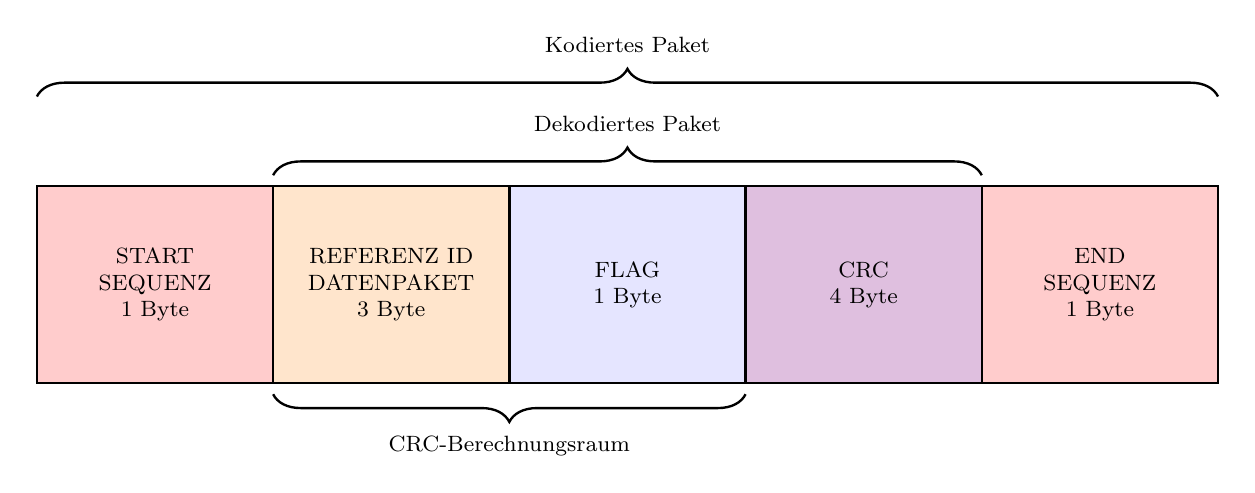
\begin{tikzpicture}[every node/.style={font=\footnotesize},every path/.style={line width=0.3mm}]

        \draw[fill=red!20] (0,0) rectangle (3,2.5) node[midway] {\parbox{3cm}{\centering START\\SEQUENZ\\1 Byte}};
        \draw[fill=orange!20] (3,0) rectangle (6,2.5) node[midway] {\parbox{3cm}{\centering REFERENZ ID\\DATENPAKET\\3 Byte}};
        \draw[fill=blue!10] (6,0) rectangle (9,2.5) node[midway] {\parbox{3cm}{\centering FLAG\\1 Byte}};
        \draw[fill=violet!25] (9,0) rectangle (12,2.5) node[midway] {\parbox{3cm}{\centering CRC\\4 Byte}};
        \draw[fill=red!20] (12,0) rectangle (15,2.5) node[midway] {\parbox{3cm}{\centering END\\SEQUENZ\\1 Byte}};

        \draw [decorate,decoration={brace,amplitude=10pt,raise=4pt},yshift=1cm]
        (0,2.5) -- (15,2.5) node [black,midway,yshift=0.8cm] {Kodiertes Paket};
        \draw [decorate,decoration={brace,amplitude=10pt,raise=4pt},yshift=0pt]
        (3,2.5) -- (12,2.5) node [black,midway,yshift=0.8cm] {Dekodiertes Paket};

        \draw [decorate,decoration={brace,amplitude=10pt,mirror,raise=4pt},yshift=0pt]
        (3,0) -- (9,0) node [black,midway,yshift=-0.8cm] {CRC-Berechnungsraum};

    \end{tikzpicture}
    \caption{Aufbau eines Kontrollpakets}
    \label{fig:controlpacket}
\end{figure}
\vspace{0.5cm}

Ein Kontrollpaket setzt sich entsprechend Abbildung \ref{fig:controlpacket} zusammen. Die referenzierte \\
Datenpaket-ID ist bei allen Kontrollblöcken, welche keine Antworten auf Datenpakete sind, Null. Das Flag Übermittelt die eigentliche Information. Die Länge des gesamten Paketes ist wegen der Kodierung zur Laufzeit möglicherweise größer, als in Abbildung \ref{fig:controlpacket} dargestellt. Eine Auflistung aller genutzten Flags erfolgt in Tabelle \ref{tab:control_flags}.

\vspace{0.5cm}
\begin{table}[H]
    \center
    \def\arraystretch{1.3}
    \rowcolors{2}{gray!15}{white}
    \begin{tabular}{|c|l|l|}
        \rowcolor{gray!50}
        \hline
        \textbf{Hex} & \textbf{Bezeichnung} & \textbf{Bedeutung}                                  \\
        \hline
        2            & close connection     & Alle Daten versandt, breit Verbindung zu schließen  \\
        4            & resend               & Inkorrektes Datenpaket erhalten, Neusenden nötig    \\
        6            & connect              & Online, bereit Verbindung aufzubauen                \\
        8            & received             & Korrektes Datenpaket erhalten, sende nächstes Paket \\
        \hline
    \end{tabular}
    \caption{Kontrollflags und ihre Bedeutung}
    \label{tab:control_flags}
\end{table}